\section*{Materials and methods}

\subsection*{Data}

Two different previously-published datasets were used here:

\begin{enumerate}

\item Diffusion MRI data from a previous study of properties of the white matter
across the lifespan\cite{yeatman2014lifespan}, containing dMRI data from 76
subjects with ages 6-50. These data were measured in a GE Discovery 750 3T MRI
scanner at the Stanford Center for Cognitive and Neurobiological Imaging. The
Stanford University IRB approved the procedures of this study. Informed consent
was obtained from each adult participant, and assent for participation was
provided by by parents/guardians for children. Voxel resolution was 2x2x2 $mm^3$
96 non-colinear directions of measurement were measured with a b=2,000 $s/mm^2$
and 30 non-colinear directions of measurement were measured with a b=1,000
$s/mm^2$. Data was preprocessed to correct for subject motion and the diffusion
tensor model \cite{basser1994mr} was fit in every voxel, using a robust fit
\cite{chang2005restore}. These data were acquired using a dual spin echo
sequence, in which there is sufficient time for eddy currents to subside between
the application of the gradients and the image acquisition, so no eddy current
correction was appliced. We will refer to this dataset as WH.

\item Diffusion MRI from from a previous study of the corticospinal tract
profile in patients with amyotrophic lateral sclerosis
(ALS)\cite{sarica2017corticospinal}, containing data from 24 ALS patients and 24
demographically matched healthy controls. These data were measured in a GE
Discovery 750 3T MRI scanner at the Institute of Bioimaging and Molecular
Physiology in Catanzaro. Informed consent was provided as approved by the
Ethical Committee of the University ``Magna Graecia'' of Catanzaro. Voxel
resolution was 2x2x2 $mm^3$ and 27 non-colinear directions were measured with a
b=1,000 $s/mm^2$. Here, both motion correction and eddy current correction were
applied before modeling the diffusioon tensor in each voxel. We will refer to
this dataset as ALS.

\end{enumerate}

Data from both of these studies was processed in a similar manner, using the
Matlab Automated Fiber Quantification toolbox (AFQ) \cite{yeatman2012tract}:
streamlines representing fascicles of white matter nerve fibers were generated
using a determinstic tractography algorithm that follows the prinicpal diffusion
direction of the diffusion tensor in each voxel (STT \cite{basser2000vivo}).
Major tracts were identified using multiple criteria: streamlines are selected
as candidates for inclusion in a bundle of streamlines that represents a tract
if they pass through known inclusion ROIs and do not pass through exclusion ROIs
\cite{wakana2007reproducibility}. In addition, a probabilistic atlas is used to
exclude streamlines which are unlikely to be part of a tract \cite{Hua2008-sh}.
Each streamline is resampled to 100 nodes and the robust mean at each location
is calculated by estimating the 3D covariance of the location of each node and
excluding streamlines that are more than 5 standard deviations from the mean
location in any node. Finally, a tract profile of tissue properties in each
tract was created by interpolating the value of MRI maps of these tissue
properties to the location of the nodes of the resampled streamlines designated
to each tract. In each of 100 nodes, the values are summed across streamlines,
weighting the contribution of each streamline by the inverse of the mahalnobis
distance of the node from the average  of that node across streamlines. This
means that streamlines that are more representative of the tract contribute more
to the tract profile, relative to streamlines that are on the edge of the tract.

This process creates tract profiles, in which diffusion measures are quantified
and averaged along twenty major fiber tracts. Here, we use only the mean
diffusivity (MD) and the fractional anisotropy (FA) of the diffusion tensor, but
additional dMRI-based maps or maps based on other quantitative MRI measurements
can also be used. These tract profiles, along with the phenotypical data we wish
to explain or predict, form the input to the SGL algorithm. In a domain-agnostic
machine learning context, the phenotypical data comprise the target variables
while the tract profiles form the feature or predictor variables (See
Fig~\ref{fig:group-structure}).

\subsection*{Sparse Group Lasso}

Before fitting a model to the data, imputation and standardization are
performed. Missing node values (e.g., in cases where AFQ designates a node as
not-a-number) are imputed via linear interpolation. Care is taken not to
interpolate across the boundaries between different tracts. Some diffusion
metrics will have naturally larger variance than others and may therefore
dominate the objective function and make the SGL estimator unable to learn from
the lower variance metrics. For example, fractional anisotropy (FA) is bounded
between zero and one and could be overwhelmed by an unscaled higher-variance
metric like the mean diffusivity (MD). To prevent this, we use the
\lstinline{StandardScaler} from scikit-learn\cite{scikit-learn}, to remove each
feature's mean and scale it to unit variance. Scaling is performed separately
within each cross-validation set's training or testing data to prevent leakage
of information between the testing and training sets\cite{kaufman2012leakage}.

After scaling and imputation, the tractometry data and target phenotypical data
can be organized in a linear model, $y = \mathbf{X} \cdot \beta$, where $y$ is
the phenotype -- categorical, such as a clinical diagnosis, or numerical, such
as the subject's age. The tractometry data is represented in the feature matrix
$\mathbf{X}$, with rows corresponding to different subjects, and columns
corresponding to diffusion measures at different nodes within each tract. The
relationship between tractometric features and the phenotypic target is
characterized by the coefficients in $\beta$. The feature matrix $\mathbf{X}$
has dimensions $N_s \times (N_t \cdot N_n \cdot N_m)$, where $N_s$ is the number
of subjects, $N_t$ is the number of white matter tracts, $N_n$ is the number of
nodes in each tract, and $N_m$ is the number of diffusion metrics calculated at
each node. Typically, $N_t = 20$, $N_n = 100$, and $2 \le N_m \le 8$, resulting
in $\mathcal{O}(10^4)$ features. Conversely, most dMRI studies have
$\mathcal{O}(10^2)$ participants, yielding a feature matrix that is wide and
short. The high dimensionality of this data requires regularization to avoid
overfitting and generate interpretable results.

In addition to regularizing the coefficients in $\beta$, we also wish to
capitalize on our knowledge of the group structure of the tract profile features
in $\mathbf{X}$. The tract-metric combinations form a natural grouping. For
example, we expect that MD features within the left arcuate fasciculus will be
correlated. Likewise for FA values within the right corticospinal tract (CST)
and so on. This group structure is represented in Fig~\ref{fig:group-structure},
which depicts the linear model $y = \mathbf{X} \cdot \beta$. Thus, we seek a
regularization approach that will fit a linear model with anatomically-grouped
covariates, where we expect to observe sparse coefficients at both the group
level and the within-group level. The sparse group lasso (SGL) is a penalized
regression technique that satisfies exactly these
criteria\cite{simon2013sparse}. It solves for a coefficient vector
$\widehat{\beta}$ that satisfies
\begin{equation}
    \widehat{\beta} = \min_\beta \frac{1}{2}
    \norm*{y - \displaystyle \sum_{\ell = 1}^{m} \mathbf{X}^{(\ell)} \cdot \beta^{(\ell)}}_2^2
    + \lambda_1 \displaystyle \sum_{\ell = 1}^{m} \sqrt{p_\ell} \norm*{\beta^{(\ell)}}_2
    + \lambda_2 \norm*{\beta}_1,
    \label{eq:sgl}
\end{equation}

where $m$ is the number of groups, $\mathbf{X}^{(\ell)}$ is the submatrix of
$\mathbf{X}$ corresponding to group $\ell$, $\beta^{(\ell)}$ is the coefficient
vector for group $\ell$ and $p_\ell$ is the length of $\beta^{(\ell)}$. The
first term is the mean square error loss, $L_{mse}$, as in the standard linear
regression framework. The second and third terms encourage groupwise sparsity
and overall sparsity, respectively. If $\lambda_1 = 0$ and $\lambda_2 = 1$, the
SGL reduces to the traditional lasso\cite{tibshirani1996regression}. Conversely,
if $\lambda_1 = 1$ and $\lambda_2 = 0$, the SGL reduces to the group
lasso\cite{yuan2006model}.

When the phenotypical target variable are categorical, as in the case of
predicting a clinical diagnosis, the SGL is readily adapted to logistic
regression, where the probability of a target variable belonging to an arbitrary
defined ``true'' class is the logistic function of the result of the linear
model,

\begin{equation}
    p(y = 1) = \frac{1}{1 + \exp(\mathbf{X}\cdot \beta)},
    \label{eq:logit}
\end{equation}

or equivalently, the mean squared error loss function in Eq~\eqref{eq:sgl} is
replaced with the cross-entropy loss, which for binary classification is the
negative log likelihood of the SGL classifier giving the ``true'' label:

\begin{equation}
    L_{mse} \rightarrow L_{\log} = -\left(y \log(p) + (1 - y) \log(1 - p)\right).
    \label{eq:logloss}
\end{equation}


\begin{figure}[!h]
    \centering
    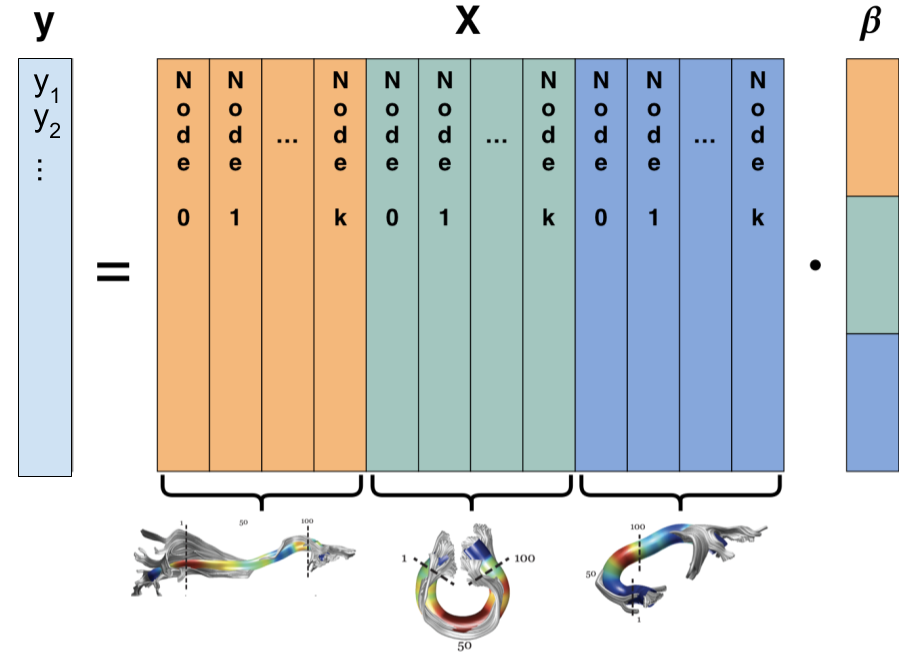
\includegraphics[width=0.65\textwidth]{dMRI_group_structure.png}
    \caption{{\bf dMRI group structure.}
        The phenotypical target data and tractometric features can be organized
    into a linear model, $y = \mathbf{X} \cdot \beta$. The feature matrix
    $\mathbf{X}$ is color-coded to reveal a natural group structure: the left
    (orange) group contains $k$ features from the inferior fronto-occipital
    fascicle (IFOF), the middle (green) group contains $k$ features from the
    corpus callosum, and the right (blue) group contains $k$ features from the
    uncinate. The coefficients in $\beta$ follow the same natural grouping.
    Fascicle images taken from Ref~\cite{yeatman2012tract}.}
    \label{fig:group-structure}
\end{figure}


\subsection*{Metaparameter optimization}

To select the values of the metaparameters $\lambda$

\begin{itemize}
  \item Computational implementation
    \begin{itemize}
      \item Insert Figure for pipeline
      \item Proximal gradient methods
      \item Meta-parameter optimization
      \item Cross-validation scheme
        \begin{itemize}
          \item Insert Figure for cross-validation scheme
        \end{itemize}
    \end{itemize}
\end{itemize}


\subsection*{Software implementation}

The full software implementation of the SGL approach presented here is available
in a Python software package called AFQ-Insight, which is developed publicly in
\url{https://github.com/richford/afq-insight}. The version of the code used to
produce the results herein is also available in XXX Zenodo DOI. AFQ-Insight
reads the target and feature data that has been processed by AFQ from comma
separated value (CSV) files conforming to the AFQ-Browser data
format\cite{yeatman2018browser} and represents them internally as
\lstinline{DataFrame} objects from the pandas Python
library\cite{mckinney2010data}. The software provides different options for
imputing missing data in the feature matrix. Missing interior nodes are imputed
using linear interpolation. For missing exterior nodes, the user may choose
between linear extrapolation and constant forward(back)-fill. Imputation uses
only values from adjacent nodes in the same white matter tract in the same
subject so there is no danger of data leakage from other subjects.